\documentclass{sig-alternate}
\usepackage{color}
\usepackage{algorithmic}
\usepackage{algorithm}
\usepackage{multirow}


%%%% User-defined macros
\newcommand{\lam}{\lambda}
\newcommand{\mycomment}[1]{\textcolor{red}{#1}}
%%%%% Uncomment the following line and comment out the previous one
%%%%% to remove all comments
%%%%% NOTE: comments still occupy a line even if invisible;
%%%%% Don't write them as a separate paragraph
%\newcommand{\mycomment}[1]{}

\begin{document}

% --- Author Metadata here ---
%%% REMEMBER TO CHANGE THE SEMESTER AND YEAR
\conferenceinfo{UMM CSci Senior Seminar Conference, December 2013}{Morris, MN}

\title{Intrusion Detection with Genetic Algorithms and Fuzzy Logic}

\numberofauthors{1}

\author{
% The command \alignauthor (no curly braces needed) should
% precede each author name, affiliation/snail-mail address and
% e-mail address. Additionally, tag each line of
% affiliation/address with \affaddr, and tag the
% e-mail address with \email.
\alignauthor
Emma Ireland\\
	\affaddr{Division of Science and Mathematics}\\
	\affaddr{University of Minnesota, Morris}\\
	\affaddr{Morris, Minnesota, USA 56267}\\
	\email{irela065@morris.umn.edu}
}

\maketitle
\begin{abstract}
This paper describes two different ways of training an intrusion detection system about possible attacks to a system: genetic algorithms and fuzzy logic. I will explain how genetic algorithms are used in intrusion detection systems and compare the results to the winning entry of the KDD99 Classifier Learning Contest. I will then explain how fuzzy genetic algorithms are used and compare those results with a decision tree algorithm.
\end{abstract}

% A category with the (minimum) three required fields
\category{}{Security and Privacy}{Intrusion Detection Systems}

\terms{Security}

\keywords{Intrusion detection, genetic algorithm, fuzzy logic, KDD99, RLD09, computer security}

\section{Introduction}
An attack on important and confidential data is a concern for many people, so it is important to have a way to detect and analyze these attacks. A way of detecting attacks is by using an intrusion detection system. An intrusion detection system is a device that monitors network activities for malicious or abnormal behaviors and then produces reports and alerts~\cite{DBLP:journals/corr/abs-1204-1336}. There are various ways of training the intrusion detection system about possible threats. Two approaches that I will talk about in this paper are the use of genetic algorithms and fuzzy logic.

In Section~\ref{sec:background} I will give some background on intrusion detection. I will explain the main types of networking attacks in Section~\ref{sec:typesAttacks}, and ways of detecting attacks in Section~\ref{sec:detectionMeth}. In Section~\ref{sec:dataSets} I will describe two data sets that are used in intrusion detection. I will explain what \emph{rules} are in Section~\ref{sec:rules}, and then give information on fuzzy logic and genetic algorithms in Sections~\ref{sec:fuzzyLogic} and~\ref{sec:GA}. After that, I will explain the measures that are used in determining the accuracy of an intrusion detection system in Section~\ref{sec:PosNeg}. In Section~\ref{sec:genAlgImp} I will explain the use of a genetic algorithm in an intrusion detection system, and in Section~\ref{sec:fuzGenAlgImp} I will explain the use of a fuzzy genetic algorithm. Section~\ref{sec:conclusion} has some conclusions about the use of genetic algorithms and fuzzy genetic algorithms in intrusion detection systems.




\section{Background}
\label{sec:background}

\subsection{Types of Networking Attacks}
\label{sec:typesAttacks}
There are four main types of networking attacks that this paper will address: \emph{denial of service}, \emph{remote to user attacks}, \emph{user to root attacks}, and \emph{probing}. Each attack that happens on a network can be placed into one of these categories.~\cite{DBLP:journals/corr/abs-1204-1336}

Denial of service (DoS) attacks happen when an attacker makes a machine inaccessible to a user by making it too busy to serve legitimate requests. For example, many systems lock out a user from an account after a certain number of failed login attempts. An attacker would be able to use this to prevent legitimate users from logging in~\cite{DoSAttacks}. Remote to user (R2L) attacks happen when an attacker sends packets to a machine over the network in order to gain access to things a local user would have on the machine. An example is when an attacker tries to gain access to a machine by guessing possible usernames and passwords. User to root (U2R) attacks happen when an attacker starts out with access on the machine and then tries to gain root access to the system. For example, if a program expects a user to input their name, the programmer has to decide how many characters that name buffer will require. Assume the program allocates 20 characters for the name buffer. Suppose the user's name has 35 characters. The last 15 characters will overflow the buffer, which could then overwrite the instructions that are to be executed next. An attacker can cause commands to be executed by manipulating the data that overflows. Probing happens when an attacker examines a machine in order to collect information about weaknesses or vulnerabilities that in the future could be used to compromise the system.~\cite{DBLP:journals/corr/abs-1204-1336, typesOfAttacks}




\subsection{Detection Methodologies}
\label{sec:detectionMeth}
There are two different ways of detecting attacks: \emph{signature-based detection} and \emph{anomaly-based detection}. 

A signature is a pattern that corresponds to a known attack. Signature-based detection compares well-known patterns of attacks that are already in the intrusion detection system against captured events in order to identify a possible attack. It is a simple and effective way to detect known attacks. Signature-based detection is also called \emph{knowledge-based detection} or \emph{misuse detection}.~\cite{Liao201316}

Anomaly-based detection looks for patterns of activity that are rare and uncommon. It is an effective way to detect new attacks. Anomaly-based detection is also called \emph{behavior-based detection}.~\cite{DBLP:journals/corr/abs-1204-1336}




\subsection{Data Sets}
\label{sec:dataSets}
Two different data sets are used in this paper: KDD99 and RLD09. The KDD99 data set is a benchmark data set that was generated by simulating a military network environment in 1999~\cite{6559603}. It has long been a standard data set for intrusion detection. The data in the set is classified as normal or attack activity. KDD99 uses 41 \emph{features}, which are properties of a \emph{record} (either an attack or normal activity), that are used to describe the activity and help to distinguish normal connections from attacks. 

In research conducted by P. Jongsuebsuk, N. Wattanapongsakorn, and
C. Charnsripinyo~\cite{6496342, 6559603}, 8 out of the 41 KDD99 features~\cite{KDD99} were used in their system:
\begin{enumerate}
  \item duration: the length of the normal or attack activity in seconds.
  \item src\_bytes: the number of bytes sent from source to destination. Source is the user who may or may not be an attacker, and destination is the server being potentially attacked.
  \item num\_failed\_logins: the number of failed login attempts.
  \item root\_shell: returns 1 if root shell is obtained, which means that the user is able to log in as root. This gives them the ability to do things like add accounts and change user passwords. If root shell is not obtained, 0 is returned.
  \item num\_access\_files: the number of operations on access control files. Access control files specify which users are granted access to objects and what operations are allowed on the objects. An example would be (Alice, delete), which would give Alice permission to delete the file.~\cite{accessControl}
  \item srv\_count: the number of connections to the same service as the current connection in the past two seconds.
  \item serror\_rate: the percentage of connections that have ``SYN" errors. When a client attempts to connect to a server, it first sends a SYN (synchronize) message to the server. The server then acknowledges the request by sending a SYN-ACK to the client. The connection is established when the client sends an ACK back to the server. A SYN error is a failure that happens early in this process.~\cite{TCP}
  \item same\_srv\_rate: the percentage of connections to the same service.
\end{enumerate}

The KDD99 data set is 14 years old, and newer attack types are not included in it because of its age. Because of this, P. Jongsuebsuk, N. Wattanapongsakorn, and
C. Charnsripinyo~\cite{6496342, 6559603} created their own data set, RLD09, to use in their experiments. To create the data set, the authors captured network data from the Computer Engineering Department at King Mongkut's University of Technology Thonburi, in Bangkok, Thailand. The data has around ten million preprocessed data \emph{packets}. A packet is a unit of data that is carried throughout a network~\cite{networkPacket}. RLD09 has 17 different types of attacks that can be divided into denial of service attacks and probe attacks. It also has normal network activity. RLD09 uses 12 features, which include the number of packets, source ports, and destination ports.




\subsection{Rules}
\label{sec:rules}
Rules are a way in which elements of one set are separated into different sets, or classes, in order to differentiate between normal connections and attacks. Rules are represented by if-then statements in the following format: If <\emph{condition}> then <\emph{action}>.~\cite{bapuji2012soft} Rules can specify the details of a packet such as the IP address, port number and protocal. If a packet matches any of the rules in the intrusion detection system then the system will take appropriate action, which may include stopping the connection or logging off the system.~\cite{DBLP:journals/corr/abs-1204-6416}




\subsection{Fuzzy Logic}
\label{sec:fuzzyLogic}
Attacks on systems do not always have a fixed pattern, so fuzzy logic is used to detect patterns that have a behavior that is between normal and unusual. A fuzzy logic rule has the following format: If <\emph{condition}> then <\emph{consequence}>, where \emph{condition} is a fuzzy variable, and \emph{consequence} is a fuzzy set. For example: if the number of packets with the same destination address is high, then the pattern is unusual. To determine what is considered high, the values of the packets are divided into fuzzy sets. In Figure~\ref{fig:triangleFigure} there are three sets: low (region A), medium (region B), and high (region C). 
\begin{figure}
\centering
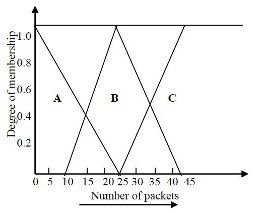
\psfig{file=triangleFigure.JPG}
\caption{Fuzzy shape with three sets: low (A), medium (B), and high (C)~\cite{DBLP:journals/corr/abs-1204-6416}}
\label{fig:triangleFigure}
\end{figure}
The x-axis are the values in the fuzzy set (number of packets), and the y-axis is the membership function, which determines the region. For example, if the number of packets with the same destination address is 15 then this will be considered as low for a degree of 0.4, but will be considered medium or high for other degrees. If the number of packets is determined to be high, then the connection will be aborted.~\cite{DBLP:journals/corr/abs-1204-6416}




\subsection{Genetic Algorithm}
\label{sec:GA}
Genetic algorithms are a search technique used to find solutions to problems. \emph{Mutation}, \emph{selection}, and \emph{crossover} are used to evolve and improve rules.

Mutation is where random bits in an \emph{individual}, or possible solution, are changed. Selection is where individuals that have a better \emph{fitness} are chosen over the other individuals. The fitness function determines the quality of a particular individual. Crossover is where two individuals swap one of their characteristics with the other to form two new individuals.

The solution to a problem is represented as a chromosome. First, a randomly generated population of chromosomes is created. According to the characteristics of the problem, the positions of each chromosome are encoded as bits, characters, or numbers. Then mutation, selection, and crossover are applied to each generation and eventually the best solution is found.~\cite{DBLP:journals/corr/abs-1204-6416}




\subsection{False Positives, False Negatives, True Positives, True Negatives}
\label{sec:PosNeg}
In a machine learning experiment, a common technique is to divide the data set into two subsets, a \emph{training set} and a \emph{testing set}. The given algorithm is then trained on the training set to look for patterns. These patterns are then verified using the test set.~\cite{bc1_ecindm} Four different measures are then used to determine the accuracy of the algorithm in question.

A \emph{false positive} (FP) happens when an intrusion detection system incorrectly identifies normal activity as being an attack. A \emph{false negative} (FN) happens when an intrusion detection system fails to identify harmful activity. A \emph{true positive} (TP) happens when an intrusion detection system correctly identifies activities to be attacks. A \emph{true negative} (TN) happens when an intrusion detection system correctly identifies activities to be normal.

The \emph{detection rate} (DR) of an intrusion detection system is the number of true positives divided by the total number of intrusions that happen.~\cite{ids}




\section{Genetic Algorithm Implementation}
\label{sec:genAlgImp}

\subsection{Algorithm Overview}
In research conducted by M. S. Hoque, M. A. Mukit, and M. A. N. Bikas~\cite{DBLP:journals/corr/abs-1204-1336}, a genetic algorithm was used to make their intrusion detection system. The system is divided into two phases: a precalculation phase and a detection phase. In the precalculation phase, a set of chromosomes are created using training data. Then this set of chromosomes is used in the detection phase for comparison. Algorithm~\ref{alg:precalc} is used in the precalculation phase.

\begin{algorithm}
\caption{Major steps in precalculation}
\label{alg:precalc}
\begin{algorithmic}
\STATE{range = 0.125}
\FOR{each training data}
  \IF{it has neighboring chromosome within range}
    \STATE{Merge it with the nearest chromosome}
  \ELSE \STATE{Create new chromosome with it}
  \ENDIF
\ENDFOR
\end{algorithmic}
\end{algorithm}

In the detection phase, a population is created for test data. Selection, crossover, and mutation occur, and then the type of the data (whether it is an attack or normal behavior) is predicted. The set of chromosomes that was created in the precalculation phase is used in the detection phase to find the fitness of each chromosome in the population. Algorithm~\ref{alg:detection} is used in the detection phase.

\begin{algorithm}
\caption{Major steps in detection}
\label{alg:detection}
\begin{algorithmic}
\STATE{Initialize the population}
\WHILE{number of generation is not reached}
  \FOR{each chromosome in the population}
    \FOR{each precalculated chromosome}
      \STATE{Find fitness // Fitness function is the standard deviation equation with distance}
    \ENDFOR
    \STATE{Assign optimal fitness as the fitness of that 
    
    chromosome}
  \ENDFOR
  \STATE{Remove some chromosomes with worse fitness}
  \STATE{Apply crossover to the selected pair of chromosomes of the population}
  \STATE{Apply mutation to each chromosome of the 
  
  population~//~mutation rate~=~0.35}
\ENDWHILE
\end{algorithmic}
\end{algorithm}




\subsection{Experimental Design and Results}
The authors of~\cite{DBLP:journals/corr/abs-1204-1336} used the KDD99 data set. They used only the numerical features of the KDD99 data set (34 out of 41 total features). For the training data set, the KDD99 10\% version file was used, and for the test data set, the KDD99 corrected version file~\cite{KDD99} was used. The training set has a total of 494,021 records, and 396,741 of them are attacks. The test set has a total of 311,029 records, and 250,436 of them are attacks. Table~\ref{tab:numberOfRecords} shows the number of records of normal and attack activity in the training and test sets.

\begin{table}
\center
\caption{Number of records}
\vspace{0.20cm}
\begin{tabular}{lll}
  & Training & Testing \\ 
Normal & 97,280 & 60,593\\
Probe  & 4,107  & 4,166\\
DoS	   & 391,458 & 229,853\\
U2R    & 52      & 228\\
R2L    & 1,124   & 16,189\\
Total  & 494,021 & 311,029\\
\end{tabular}
\center
\label{tab:numberOfRecords}
\end{table}


\begin{table*}
\center
\caption{Results for Genetic Algorithm Experiment}
\vspace{0.20cm}
\begin{tabular}{cccccccc}
& & \multicolumn{5}{ c }{Predicted label} \\ 
& & Normal & Probe & DoS & U2R & R2L & \% Correct \\ \cline{3-8}
\multicolumn{1}{ c }{\multirow{2}{*}{Actual class} } &
\multicolumn{1}{ c| }{Normal} & 42138 & 1421 & 15835 & 486 & 713 & 69.5\\
\multicolumn{1}{ c  }{}                        &
\multicolumn{1}{ c| }{Probe} & 398 & 2963 & 654 & 2 & 149 & 71.1   \\
\multicolumn{1}{ c  }{\multirow{2}{*}{} } &
\multicolumn{1}{ c| }{Dos} & 921 & 432 & 228489 & 1 & 10 & 99.4\\
\multicolumn{1}{ c  }{}                        &
\multicolumn{1}{ c| }{U2R} & 146 & 21 & 8 & 43 & 10 & 18.9\\
\multicolumn{1}{ c  }{}                        &
\multicolumn{1}{ c| }{R2L} & 11191 & 578 & 3398 & 141 & 881 & 5.4\\

\multicolumn{1}{ c  }{}                        &
\multicolumn{1}{ c| }{} &  &  &  &  &  & \\

\multicolumn{1}{ c  }{\% Correct}                        &
\multicolumn{1}{ c| }{} & 76.9 & 54.7 & 92.0 & 6.4 & 50.0 \\
\end{tabular}
\center
\label{tab:genAlgResults}
\end{table*}


\begin{table*}
\center
\caption{Results for Genetic Algorithm Experiment}
\vspace{0.20cm}
\begin{tabular}{cccc}
%\cline{3-8}
& & \multicolumn{2}{ c }{Predicted label} \\ 
& & Normal & Intrusion\\ \cline{3-4}
\multicolumn{1}{ c }{\multirow{2}{*}{Actual class} } &
\multicolumn{1}{ c| }{Normal} & True Negative (42,138) & False Positive (18,455)\\
\multicolumn{1}{ c  }{}                        &
\multicolumn{1}{ c| }{Probe} & False Negative (12,528) & True Positive (237,908)\\
\end{tabular}
\center
\label{tab:genAlgResults2}
\end{table*}


In the detection phase, an initial population is created and then is compared with each chromosome that was created in the precalculation phase. Crossover and mutation happen in the population in order to create a new population. The results from running the genetic algorithm are shown in Tables~\ref{tab:genAlgResults} and~\ref{tab:genAlgResults2}. The detection rate was 94.9\%. The false positive rate was 30.5\%. The false negative rate was 5\%. The true negative rate was 69.5\%.

The authors of~\cite{DBLP:journals/corr/abs-1204-1336} compared their results with the winning entry of the KDD99 Classifier Learning Contest~\cite{KDD99Contest}, and found that they had a better detection rate for denial of service and user to root attacks than the winning entry.




\section{Fuzzy Genetic Algorithm Implementation}
\label{sec:fuzGenAlgImp}
The focus of~\cite{6496342, 6559603} is on detecting new or unknown types of attacks in a network. The intrusion detection system used is able to identify normal network activity as well as attacks using a fuzzy genetic algorithm. This kind of algorithm is able to learn new attacks, and has a high detection rate. 




\subsection{Fuzzy Algorithm}
In order to measure the probability that a record is an attack, a trapezoidal shape was used in the algorithm. This is shown in Figure~\ref{fig:trapFigure}. The trapezoidal shape has four parameters: $a, b, c$, and $d$. Algorithm~\ref{alg:fuzAlg} calculates the probability of a record being an attack.

\begin{figure}
\centering
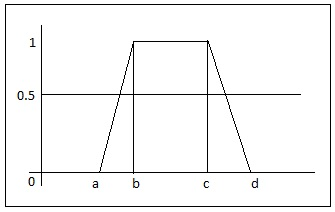
\psfig{file=trapFigure.jpg}
\caption{Trapezoidal shape with 4 parameters where $a\leq b\leq c\leq d$}
\label{fig:trapFigure}
\end{figure}

\begin{algorithm}
\caption{Fuzzy Algorithm}
\label{alg:fuzAlg}
\begin{algorithmic}
\IF{data value is between $b$ and $c$}
  \STATE{prob = 1.0}
\ELSIF{data value is between $a$ and $b$}
  \STATE{
    prob = $(\textrm{data}-a)/(b-a)$
  }
\ELSIF{data value is between $c$ and $d$}
  \STATE{
    prob = $(d-\textrm{data})/(d-c)$
  }
\ELSE \STATE{prob = 0.0}
\ENDIF
\end{algorithmic}
\end{algorithm}

The four parameters a, b, c, and d are encoded into blocks of binary strings, where each block is a feature with values between 0.0 and 7.0. See Figure~\ref{fig:fuzEncodingForFeature} for an example of a block. A rule has 12 blocks of features, and at the end of the string is the type of attack. An example of this is Figure~\ref{fig:rule}.

\begin{figure}
\centering
\caption{Fuzzy encoding for a feature}
\vspace{0.20cm}
\begin{tabular}{|cccc|} \hline
010 & 011 & 100 & 101\\
a=2 & b=3 & c=4 & d=5\\
\hline\end{tabular}
\label{fig:fuzEncodingForFeature}
\end{figure}

\begin{figure*}
\centering
\caption{A rule with 12 blocks of features}
\vspace{0.20cm}
\begin{tabular}{|cccc|c|cccc|c|} \hline
010 & 011 & 100 & 101   & ...... & 010 & 011 & 101 & 111   & DoS\\
a=2 & b=3 & c=4 & d=5   & ...... & a=2 & b=3 & c=5 & d=7   &\\ 
    &     & Block 1&    &        &     & Block 12& &       & Type\\
\hline\end{tabular}
\label{fig:rule}
\end{figure*}




\subsection{Algorithm Overview}
The algorithm that is used in~\cite{6496342, 6559603} first randomly generates rules. Then the rules are improved in the training phase, which can be seen in Algorithm~\ref{alg:fuzGenAlg}. After that, the rules are used to classify the data in the testing phase. Algorithm~\ref{alg:fuzGenAlg} describes the fuzzy genetic algorithm that is used. One record (either an attack or normal activity) is passed into a rule. Each feature in a record is matched to one block of the rule. The parameters of each block measure the probability of an attack using the trapezoidal fuzzy rule shape. The probabilities of each block are then compared with a threshold to determine if the record represents an attack or normal behavior.

\begin{algorithm}
\caption{Fuzzy Genetic Algorithm}
\label{alg:fuzGenAlg}
\begin{algorithmic}
\FOR{each record}

  \FOR{each rule}
    \FOR{each feature}
      \STATE{prob = fuzzy(); // Algorithm~\ref{alg:fuzAlg}}
      \STATE{totalprob = totalprob + prob;}
    \ENDFOR
    
    \IF{totalprob > threshold} 
      \STATE{class is attack;}
      \ELSE \STATE{class is normal;}
    \ENDIF
  \ENDFOR
  
  \STATE{compare the predicted result with actual result}
  \STATE{find $A$, $B$, $\alpha$, and $\beta$}
  \STATE{// $A$ is total number of attack records. $B$ is total number of normal records. $\alpha$ is total number of attack records correctly identified as attack. $\beta$ is total number of normal records incorrectly classified as attack.}
\ENDFOR
\STATE{calculate fitness}
\STATE{//create next generation}
\STATE{preserve\_best()}
\STATE{crossover()}
\STATE{mutation() // mutation rate~=~0.30}
\end{algorithmic}
\end{algorithm}


The fitness function to be maximized is:
\begin{equation*}
\textrm{fitness function} = \frac{\alpha}{A} - \frac{\beta}{B}
\end{equation*}
$A$ is total number of attack records. $B$ is total number of normal records. $\alpha$ is total number of attack records correctly identified as attack. $\beta$ is total number of normal records incorrectly classified as attack.

In this implementation, a population size of 10 was used for each generation. An individual in the population represents a possible detection rule. The two best individuals from a present generation are preserved for the next generation. The other individuals in the new generation come from mutation and single-point crossover.




\subsection{Experimental Design and Results}

\subsubsection{Experiments using Only RLD09}
The experiments that the authors of~\cite{6496342, 6559603} performed used a total of 16,000 records of normal activity and 10,500 records of attack activity. Of the attack records, 4,000 of them were denial of service attacks and 6,500 were probe attacks.

In the first experiment, the fuzzy genetic algorithm was used to create denial of service and probe detection rules and then the rules were verified with known attack types. 10,000 records were used for the training set and all 26,500 records were used for the testing set. The two steps in the training process were to find a denial of service rule, and find a probe rule. Both of these rules were then used together in the testing process to identify attacks from the testing data set.

The detection rate of denial of service attacks in training was 91.64\% and the detection rate of probe attacks in training was 94.79\%. The detection rate of the testing data set increased to 97.92\%. Results from this experiment are shown in Table~\ref{tab:fuzGenExp1}.

\begin{table*}
\center
\caption{Results from Experiment 1}
\vspace{0.20cm}
\begin{tabular}{ccccccc}
 & Attack & Normal & Total Records & FP (\%) & FN (\%) & DR (\%)\\
DoS Training & 1499 & 8501 & 10000 & 1.46 & 47.50 & 91.64\\
Probe Training & 2496 & 7504 & 10000 & 1.83 & 15.38 & 94.79\\
Testing & 10500 & 16000 & 26500 & 1.13 & 4.10 & 97.92\\
\end{tabular}
\label{tab:fuzGenExp1}
\center
\end{table*}

In the second experiment, seven tests were run. For each test case there were 13 attack types plus normal activity that were in the training data set. Three attack types were used for the unknown testing data set. For example, test case 1 used the training data set that does not have Advance Port Scan, Ack Scan, and Xmas Tree, which are all probe attacks. These three attacks were then used for the testing data set. Table~\ref{tab:fuzGenExp2} shows some of the results from the fuzzy genetic algorithm and a decision tree algorithm, which is another common way of addressing these problems. For further information on decision trees, see~\cite{decisionTree}. When compared with the decision tree algorithm, the fuzzy genetic algorithm has a higher detection rate in all cases except 3 and 5. It can be seen that in cases 2 and 4 the decision tree has low detection rates, while the fuzzy genetic algorithm has much higher detection rates.


\begin{table}
\caption{Unknown Attack Experiment}
\vspace{0.20cm}
\begin{tabular}{llll}
Test & Unknown & Decision & Fuzzy\\
Case & Attacks & Tree DR (\%)  & Genetic DR (\%)\\ \hline

1 & Adv Port Scan (Probe) & Avg = & Avg =\\
  & Ack Scan (Probe)		  & 98.33 & 100\\
  & Xmas Tree (Probe)		  &		  &\\ \hline

2 & UDP Flood (DoS) & Avg = & Avg =\\
  & Host Scan (Probe) & 46.65 & 99.80\\
  & UDP Scan (Probe)  &       &\\ \hline

3 & Jping (DoS)    & Avg =          & Avg =\\
  & Syn Scan (Probe) & 99.70 & 98.75\\
  & Fin Scan (Probe) &                &\\ \hline

4 & UDP Flood (DoS) & Avg = & Avg =\\
  & RCP Scan (Probe)  & 70.35 & 98.15\\
  & Fin Scan (Probe)  &       &\\ \hline

5 & Http Flood (DoS) & Avg =          & Avg =\\
  & RCP Scan (Probe)  & 99.94 & 97.50\\
  & Fin Scan (Probe) &                &\\
\hline\end{tabular}
\label{tab:fuzGenExp2}
\end{table}




\subsubsection{Experiments using Both RLD09 and KDD99}
The authors of~\cite{6496342, 6559603} also ran experiments that used and compared the RLD09 data set with the KDD99 data set. They used the KDD99 10\% version file~\cite{KDD99} for both the training dataset and testing dataset.

The authors of~\cite{6496342, 6559603} first trained and tested the fuzzy genetic algorithm (Algorithm~\ref{alg:fuzGenAlg}) with the KDD99 data set. There were 6 different types of denial of service attacks and 4 different types of probe attacks. The detection rate of the KDD99 data set was 98.72\%. Then 26,500 records of the RLD09 data set were used as the training set. The detection rate was 97.97\%. The results of this experiment are shown in Table~\ref{tab:bothSetsResults}.

\begin{table}
\caption{KDD99 and RLD09 Results}
\vspace{0.20cm}
\begin{tabular}{cccccc}
Data set & Attack & Normal & FP (\%) & FN (\%) & DR (\%)\\ \hline
KDD99 & 160,117 & 39,337 & 0.13 & 1.55 & 98.72\\
RLD09 & 10,500 & 16,000 & 1.14 & 3.39 & 97.97\\
\end{tabular}
\label{tab:bothSetsResults}
\end{table}

The next experiment was the use of the KDD99 training set with the fuzzy genetifc algorithm to separate the data into two classes. Then each specific attack type was extracted and combined with normal activity. Ten tests were run, and Table~\ref{tab:kddAttacks} shows the accuracy of detecting some of the cases. The results showed that the detection rate of most of the cases were greater than 93\%. The results also showed that the behavior of the attacks were highly distinctive from normal activity. There were only two cases that had low detection rates, one of which is case 1 in Table~\ref{tab:kddAttacks}.

\begin{table}
\caption{Results for KDD99 with Certain Attacks}
\vspace{0.20cm}
\begin{tabular}{cccccc}
Test & Attack & Type & FP (\%) & FN (\%) & DR (\%)\\ \hline
1 & Back & DoS & 85.33 & 0.00 & 16.56\\
2 & Smurf & DoS & 0.76 & 0.10 & 99.73\\
3 & Portsweep & Probe & 6.40 & 0.00 & 93.66\\
4 & Satan & Probe & 0.74 & 3.75 & 99.22\\
\end{tabular}
\label{tab:kddAttacks}
\end{table}

The final experiment that was run used only the RLD09 data set with the fuzzy genetic algorithm. 17 tests were run, and Table~\ref{tab:rldAttacks} shows the accuracy of detecting some of the cases. The results showed that the detection rate of a majority of the cases were greater than 97.5\%. Again, there were only two test cases that had low detection rates, one of which is case 2 in Table~\ref{tab:rldAttacks}.

\begin{table}
\caption{Results for RLD99 with Certain Attacks}
\vspace{0.20cm}
\begin{tabular}{cccccc}
Test & Attack & Type & FP (\%) & FN (\%) & DR (\%)\\ \hline
1 & Smurf & DoS & 0.02 & 0 & 99.98\\
2 & UDP Flood & DoS & 11.06 & 0 & 89.59\\
3 & Ackscan & Probe & 0.03 & 0 & 99.97\\
4 & Synscan & Probe & 0.65 & 4.2 & 99.24\\
\end{tabular}
\label{tab:rldAttacks}
\end{table}




\section{Conclusions}
\label{sec:conclusion}
This paper showed that the use of genetic algorithms and fuzzy logic in intrusion detection are effective ways of detecting attacks. The genetic algorithm that was used in~\cite{DBLP:journals/corr/abs-1204-1336} had a high detection rate for denial of service attacks. When compared with the winning entry of the KDD99 Classifier Learning Contest, it was shown to have a better detection rate for both denial of service and user to root attacks. The fuzzy genetic algorithm that was used in~\cite{6496342, 6559603} had a higher detection rate than a decision tree algorithm in most cases. It was also shown that fuzzy genetic algorithms are good at detecting unknown attacks. 



%\section{Acknowledgments}




% The following two commands are all you need in the
% initial runs of your .tex file to
% produce the bibliography for the citations in your paper.
\bibliographystyle{abbrv}
% sample_paper.bib is the name of the BibTex file containing the
% bibliography entries. Note that you *don't* include the .bib ending here.
\bibliography{annotated_bibliography}  
% You must have a proper ".bib" file
%  and remember to run:
% latex bibtex latex latex
% to resolve all references

\end{document}
